%!TEX root = ../TAMUTemplate.tex
%%%%%%%%%%%%%%%%%%%%%%%%%%%%%%%%%%%%%%%%%%%%%%%%%%%
%
%  New template code for TAMU Theses and Dissertations starting Fall 2016.
%
%
%  Author: Sean Zachary Roberson 
%	 Version 3.16.09
%  Last updated 9/12/2016
%
%%%%%%%%%%%%%%%%%%%%%%%%%%%%%%%%%%%%%%%%%%%%%%%%%%%

%%%%%%%%%%%%%%%%%%%%%%%%%%%%%%%%%%%%%%%%%%%%%%%%%%%%%%%%%%%%%%%%%%%%%%
%%                           APPENDIX A
%%%%%%%%%%%%%%%%%%%%%%%%%%%%%%%%%%%%%%%%%%%%%%%%%%%%%%%%%%%%%%%%%%%%%

\phantomsection

\chapter{\texorpdfstring{\uppercase{History of the Standard Model}}{History of the Standard Model}}
\label{appendix:standard_model_history}

During its tenure, the standard model has provided a remarkably accurate description of results from both accelerator and non-accelerator experiments.
In fact, all of the standard model particles shown in~\ref{fig:standard_model} have been observed and measured, most of these discoveries taking place in the last sixty years.
The original quark model proposed by Gell-Mann and Zweig in 1964 only included the up, down, and strange quarks.
The up and down quarks were later observed by deep inelastic scattering experiments at the Stanford Linear Accelerator (SLAC), which by extension proved the existence of the strange quark.
The charm quark was proposed by Bj{\o}rken and Glashow also in 1964~\cite{BJORKEN1964255}, but is credited to Sheldon Lee Glashow, John Iliopoulos, and Luciano Maianiafter they proposed the Glashow–Iliopoulos–Maiani (GIM) mechanism in 1970~\cite{PhysRevD.2.1285}.
The charm quark was later observed in \JPsi decays by SLAC~\cite{PhysRevLett.33.1406} and Brookhaven National Laboratory (BNL)~\cite{PhysRevLett.33.1404}.
The invariant distribution presented in the original BNL paper can be found in figure~\ref{fig:JPsiInvariantMass}.
The bottom or beauty quark was later proposed by Kobayashi and Maskawa in 1973~\cite{doi:10.1143/PTP.49.652} and observed by the E288 experiment led by Leon Lederman at the Fermi National Accelerator Laboratory (FNAL) in 1977~\cite{PhysRevLett.39.252}.
Kobayashi and Maskawa were trying to describe CP violation in the weak interaction, finally earning a Nobel prize for their work in 2008.

Following this flurry of quark discoveries, the \W and \Z bosons were observed at CERN in 1983 in proton-antiproton collisions of \CM{540}\gev at the Super Proton Synchroton (SPS).
This was research lead by Carlo Rubbia using the UA1 experiment~\cite{1983398} and Pierre Darriulat on the UA2 experiment~\cite{BAGNAIA1983130}.
The invariant mass of the \Z boson as seen by UA2 is shown in figure~\ref{fig:ZeeInvariantMass}.
While an insufficient number of \W bosons were observed to make precision measurements, this was accomplished using Large Electron-Positron Collider (LEP) experiment, also at CERN, where the \W and \Z masses were measured to be:
\begin{align}
\begin{split}
	\MZ &= \joinsym{91.1875}{\pm}{0.0021}\gev\\
	\MW &= \joinsym{80.376}{\pm}{0.0033}\gev
\end{split}
\end{align}
Finishing off an amazing 30 years of discoveries and completing the third and final generation of quarks predicted by Kobayashi and Maskawa, the top quark was jointly discovered in 1995 by the CDF~\cite{PhysRevLett.74.2626} and D0~\cite{PhysRevLett.74.2422} experiments at FNAL using the \CM{1.4}\tev Tevatron accelerator.
Its mass was measured to be \joinsym{\Mt}{\sim}{176}\gev.

\begin{figure}[!hbt]
    \centering
    \begin{subfigure}[t]{0.48\textwidth}
        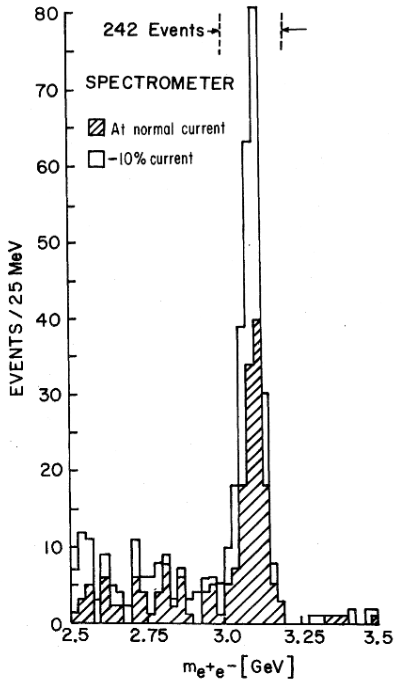
\includegraphics[width=\textwidth]{\figpath/Appendix1/JPsiInvariantMass.png}
        \caption{The invariant mass spectrum of the \JPsi particle discovered at BNL~\cite{PhysRevLett.33.1404}.}
        \label{fig:JPsiInvariantMass}
    \end{subfigure}
    \begin{subfigure}[t]{0.48\textwidth}
        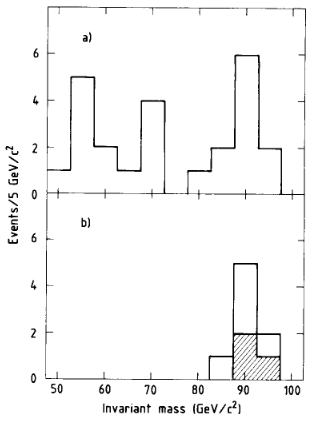
\includegraphics[width=\textwidth]{\figpath/Appendix1/ZeeInvariantMass.png}
        \caption{The invariant mass spectrum of the $\Z{\rightarrow}\Pep\Pem$ decay as seen by the UA2 collaboration. The upper half of the figure shows the number of events with a calorimeter cluster while the lower half shows the eight events that mad it past all selection criteria~\cite{BAGNAIA1983130}.}
        \label{fig:ZeeInvariantMass}
    \end{subfigure}
    \caption{Invariant mass distributions from the discoveries of the \JPsi meson and \Z boson.}
    \label{fig:JPsiAndZ}
\end{figure}

At this point in time, the Higgs boson was the final particle left to be discovered.
Both LEP and the Tevatron failed to observe the particle, though CDF and D0 were able to exclude all masses for the Higgs boson except in the ranges \range{115}{\MH}{155}\gev and \joinsym{\MH}{>}{176}\gev as seen in fig~\ref{fig:TevatronHiggsExclusions}~\cite{PhysRevD.88.052014}.
The 2012 Higgs boson discovery was jointly announced by the CMS and ATLAS collaborations at CERN~\cite{201230,20121}.
By combining the 5.1\fbinv of 7\tev data and 19.7\fbinv of 8\tev data, CMS was able to uses the $\PH{\rightarrow}\GG$ and $\PH{\rightarrow}\ZZ^{*}{\rightarrow}4\ell$ channels to measure the mass to be \longmassasym{125.3}{0.27}{0.26}{0.15}{0.15}{\gev} as shown in fig.~\ref{fig:HiggsMassBestFit}~\cite{Khachatryan2015}.
Figs.~\ref{fig:HGammaGammaPeak} and~\ref{fig:HZZPeak} show the invariant mass distributions for the diphoton and four-lepton systems obtained by the CMS experiment.
The cross section $\sigma$ was found to be consistent with that of the standard model such that the signal strength at the measured mass was found to be
\begin{equation}
\frac{\sigma}{\sigma_{SM}}=\text{1.00}\pm\text{0.09}\stat_{-\text{0.07}}^{+\text{0.08}}\theory\pm\text{0.07}\syst
\end{equation}
A graphical representation of this can be found in fig.~\ref{fig:HiggsSignalStrength}.
Measurements of other properties such as spin, parity, production rates, and the ratio of couplings to fermions and vector bosons are discussed in~\cite{Khachatryan2015}.

\begin{figure}[!hbt]
    \centering
    \begin{subfigure}[t]{0.48\textwidth}
        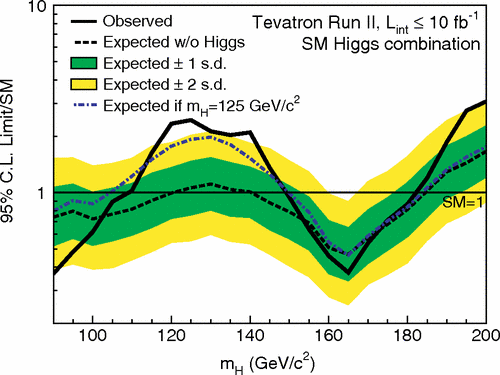
\includegraphics[width=\textwidth]{\figpath/Appendix1/TevatronHiggsExclusions.png}
        \caption{}
        \label{fig:TevatronHiggsExclusions}
    \end{subfigure}
    \begin{subfigure}[t]{0.48\textwidth}
        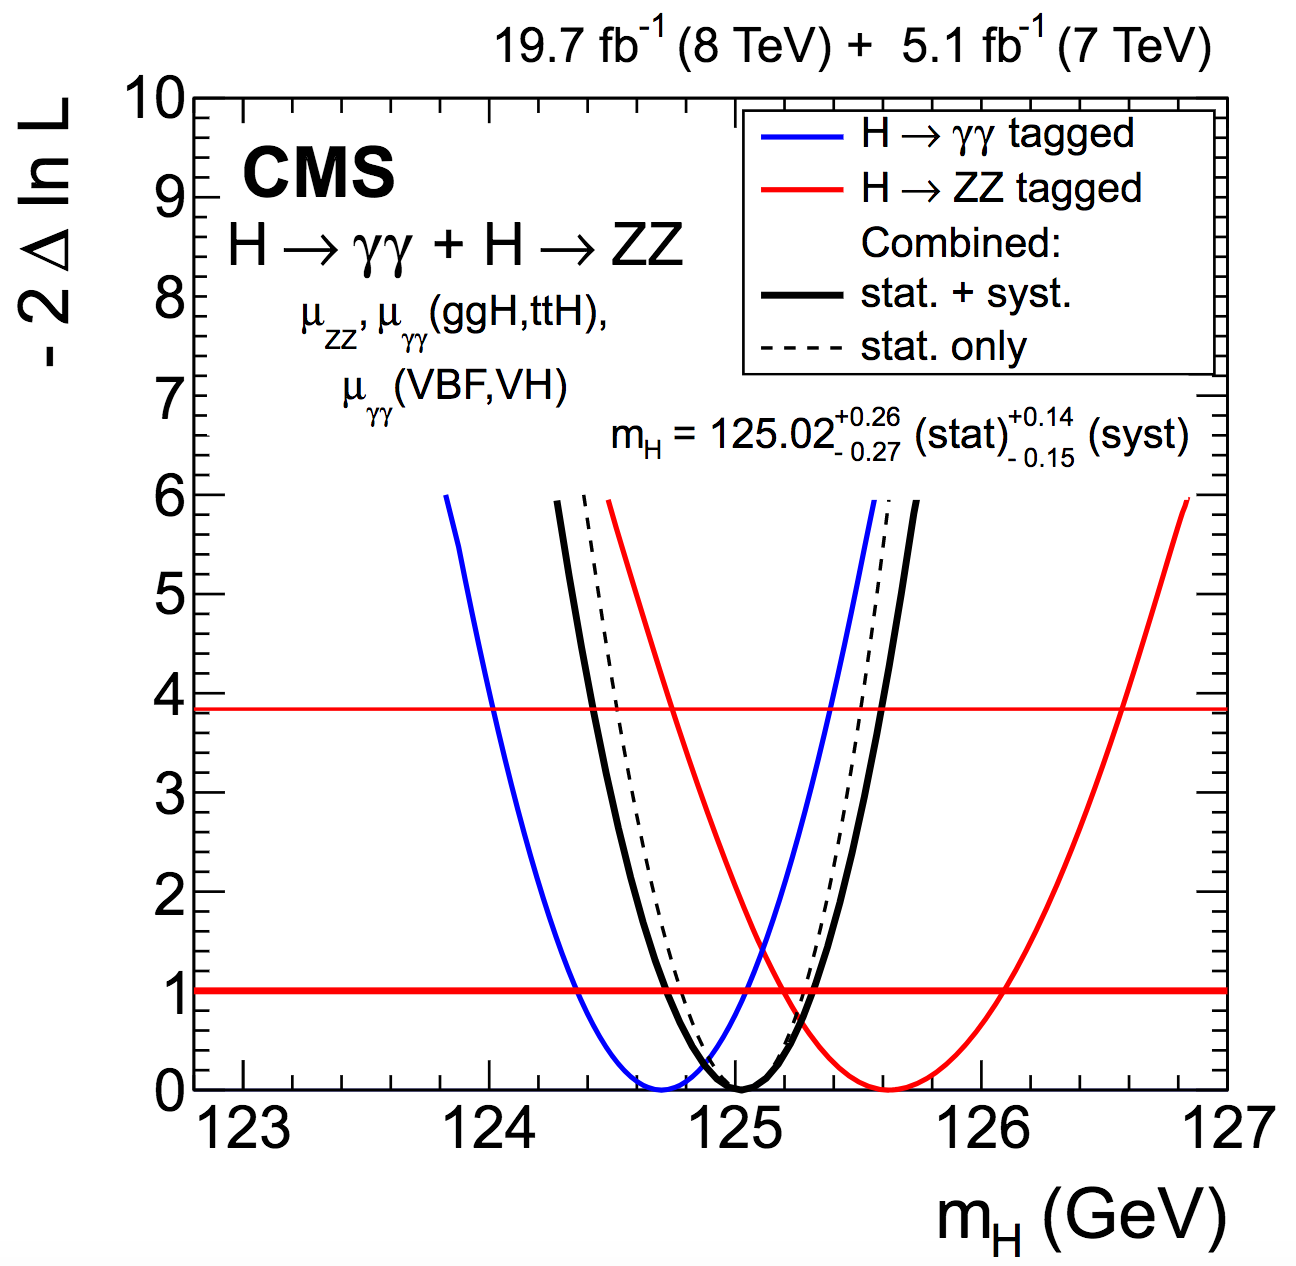
\includegraphics[width=\textwidth]{\figpath/Appendix1/HiggsMassBestFit.png}
        \caption{}
        \label{fig:HiggsMassBestFit}
    \end{subfigure}

    \begin{subfigure}[t]{0.52\textwidth}
        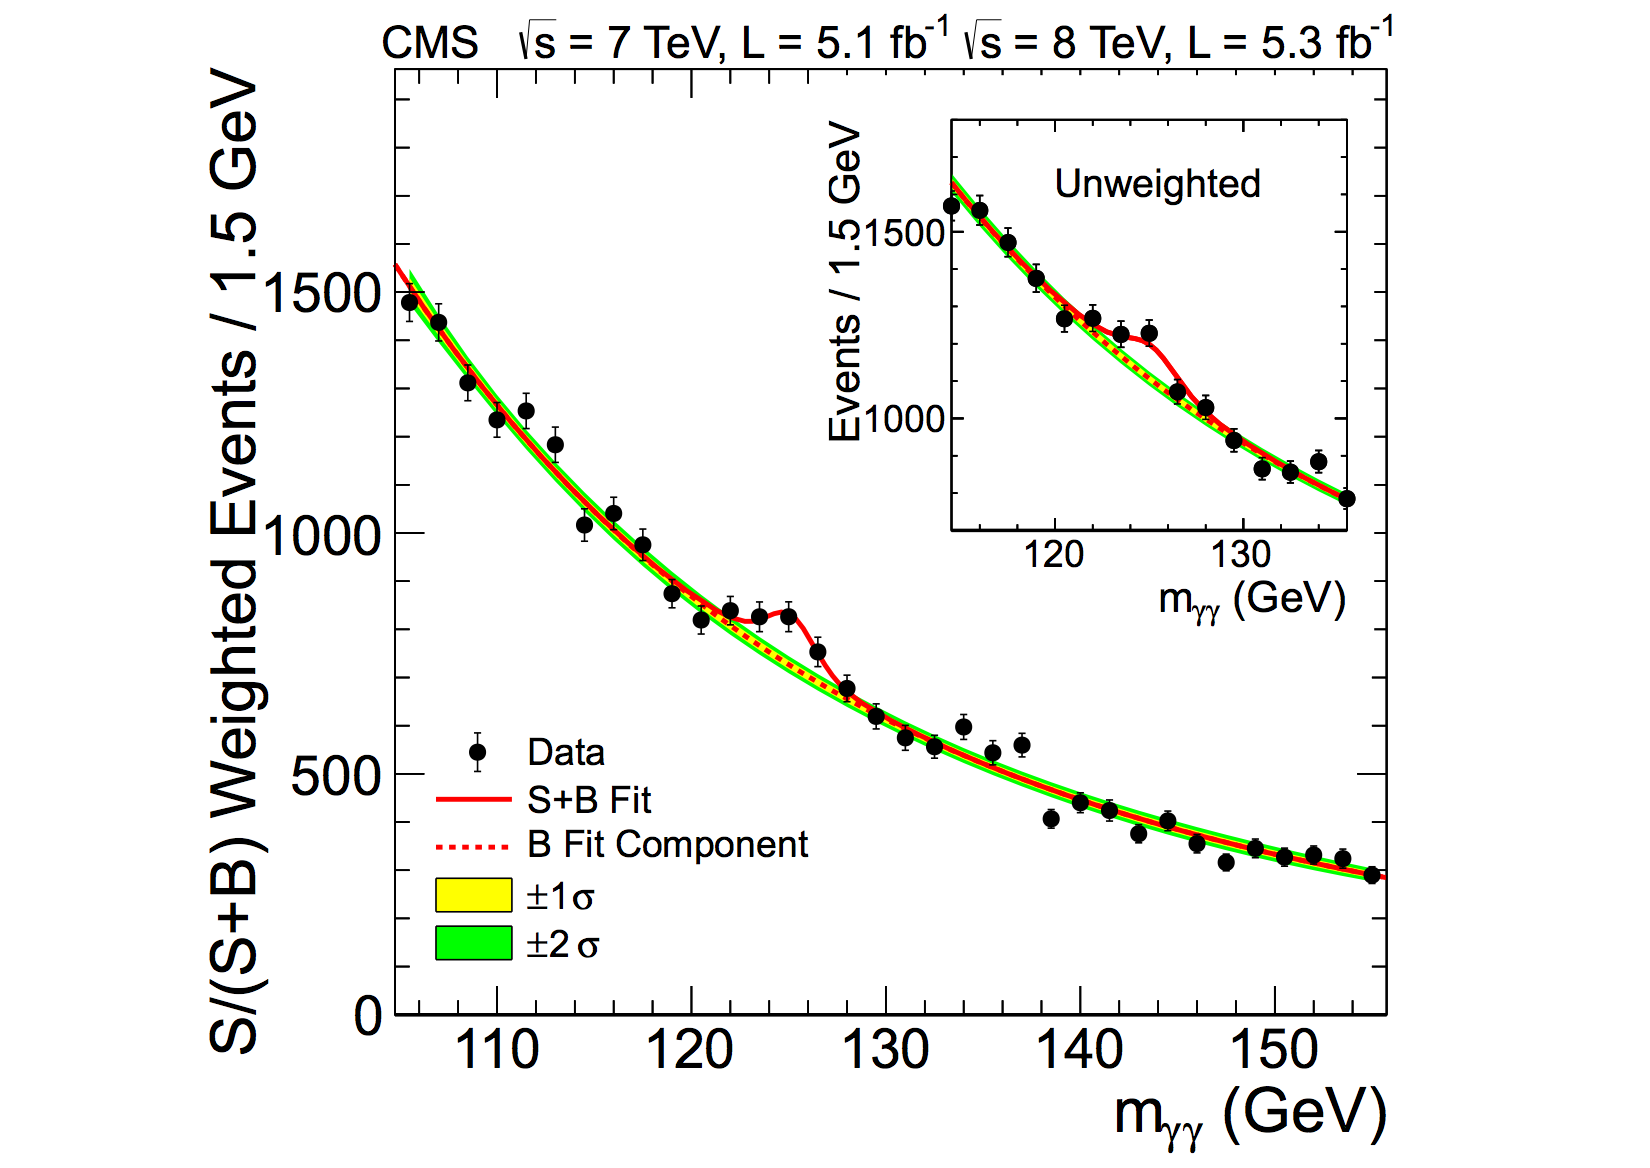
\includegraphics[width=\textwidth]{\figpath/Appendix1/HGammaGammaPeak.png}
        \caption{}
        \label{fig:HGammaGammaPeak}
    \end{subfigure}
    \begin{subfigure}[t]{0.44\textwidth}
        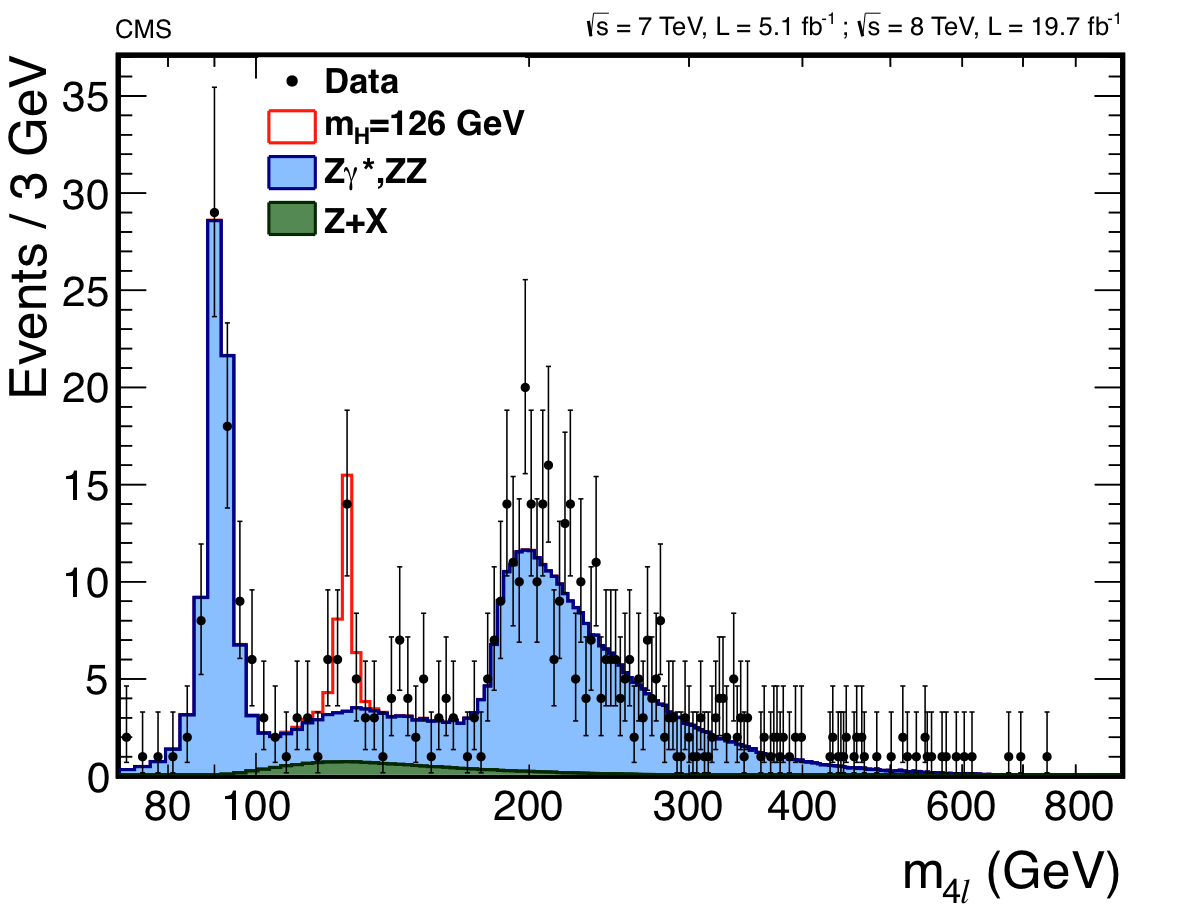
\includegraphics[width=\textwidth]{\figpath/Appendix1/HZZPeak.png}
        \caption{}
        \label{fig:HZZPeak}
    \end{subfigure}
    \caption{Key figures showing the Higgs boson discovery in two high-resolution channels. (a) The combined CDF and D0 exclusion plot for the Higgs mass before the discovery~\cite{PhysRevD.88.052014}. (b) The best fit mass results from the \GG and \ZZ decay channels at CMS~\cite{201230}. (c) The diphoton invariant mass distribution. The black markers represent the data, the solid and dashed red lines represent the fitted signal and background, and the colored bands represent the $\pm1$ and $\pm2$ standard deviation uncertainties in the background estimate. The major canvas shows each event weighted by the $\frac{S}{S+B}$ value of its selection category. (d) The four-lepton invariant mass distribution where the black markers are the data, the filled histograms show the background estimates, and the open histogram shows the background plus signal expectation for a Higgs boson mass of $\MH=125\gev$.}
    \label{fig:HiggsDiscovery}
\end{figure}

\begin{figure}[!hbt]
    \centering
    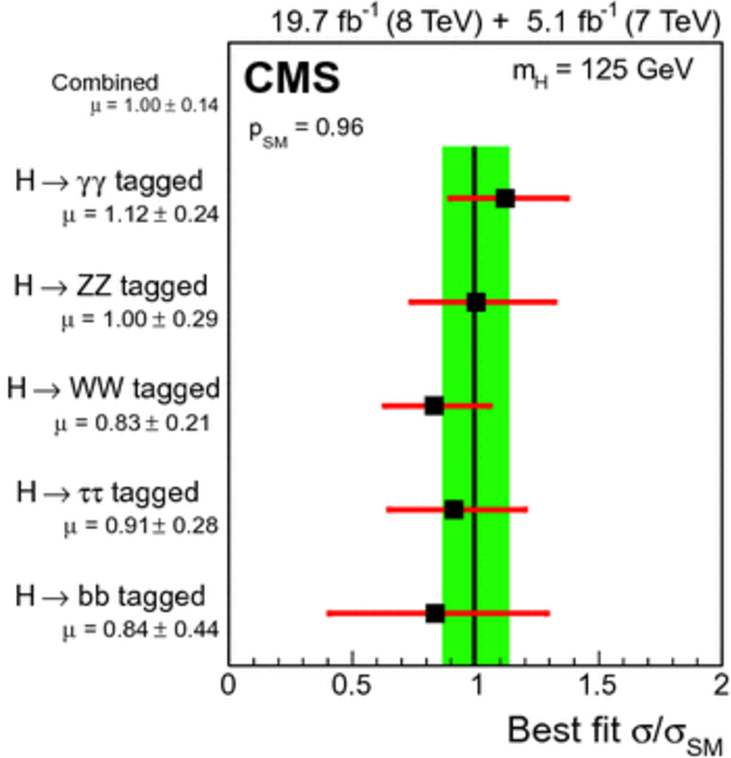
\includegraphics[width=0.95\textwidth]{\figpath/Appendix1/10052_2015_3351_Fig4_HTML.pdf}
    \caption{Best-fit $\sigma/\sigma_{SM}$ grouped by predominant decay mode. The vertical band is the overall combined analysis value and the horizontal bars show the $\pm$1 uncertainties (statistical and systematic)~\cite{Khachatryan2015}.}
	\label{fig:HiggsSignalStrength}
\end{figure}
In the past, the experimental measurements of electroweak precision observables at LEP, SLAC, the Tevatron, and the LHC have been paired with very accurate theoretical predictions.
The benefit of these observables is that they can probe energy scales beyond what is capable through direct measurements by accounting for the effects of higher order corrections.
Free parameters in the Standard Model could be constrained by doing global fits of the electroweak sector.
Now that the Higgs boson has been found, and assuming this is the SM Higgs boson, the fit is over-constrained because all parameters used in the fit are known.
Instead of constraining the free parameters we are now able to test the consistency of the Standard Model and even predict some parameters to higher precision than we are currently able to measure.

These complicated fits are performed by several groups~\cite{ckmfitter,gfitter,zfitter,lepewwg}, but only the results from the GFitter group~\cite{Baak:2014ora,Flacher:2008zq} will be used here.
Some of the measurements included in the fits are of the mass of the Higgs boson, the mass and widths of the \W and \Z bosons, the masses of the top, botton, and charm quarks, the strong coupling constant, the weak mixing angle, among others.
Figure~\ref{fig:SMConsistency} shows the comparison of the fit results with the direct measurements of the parameters, all of which agree to within $3\sigma$.
A common test of the Standard Model is to independently measure the top quark and W boson masses.
Figure~\ref{fig:mWmtGFitter} shows the 68\% and 95\% confidence level intervals obtained for \MW versus \Mt for the case where the direct Higgs mass measurement is included (blue) and excluded (grey). In both cases the fits agree with the direct measurements shown in the green bands and ellipses.
Figure~\ref{fig:mWthetaEffGFitter} shows the corresponding plot for the \W boson mass and the effective weak mixing angle.
In all cases the fit procedure agrees with the direct measurements, showing the consistency of the Standard Model within current experimental precision.

\begin{figure}[!hbt]
    \centering
    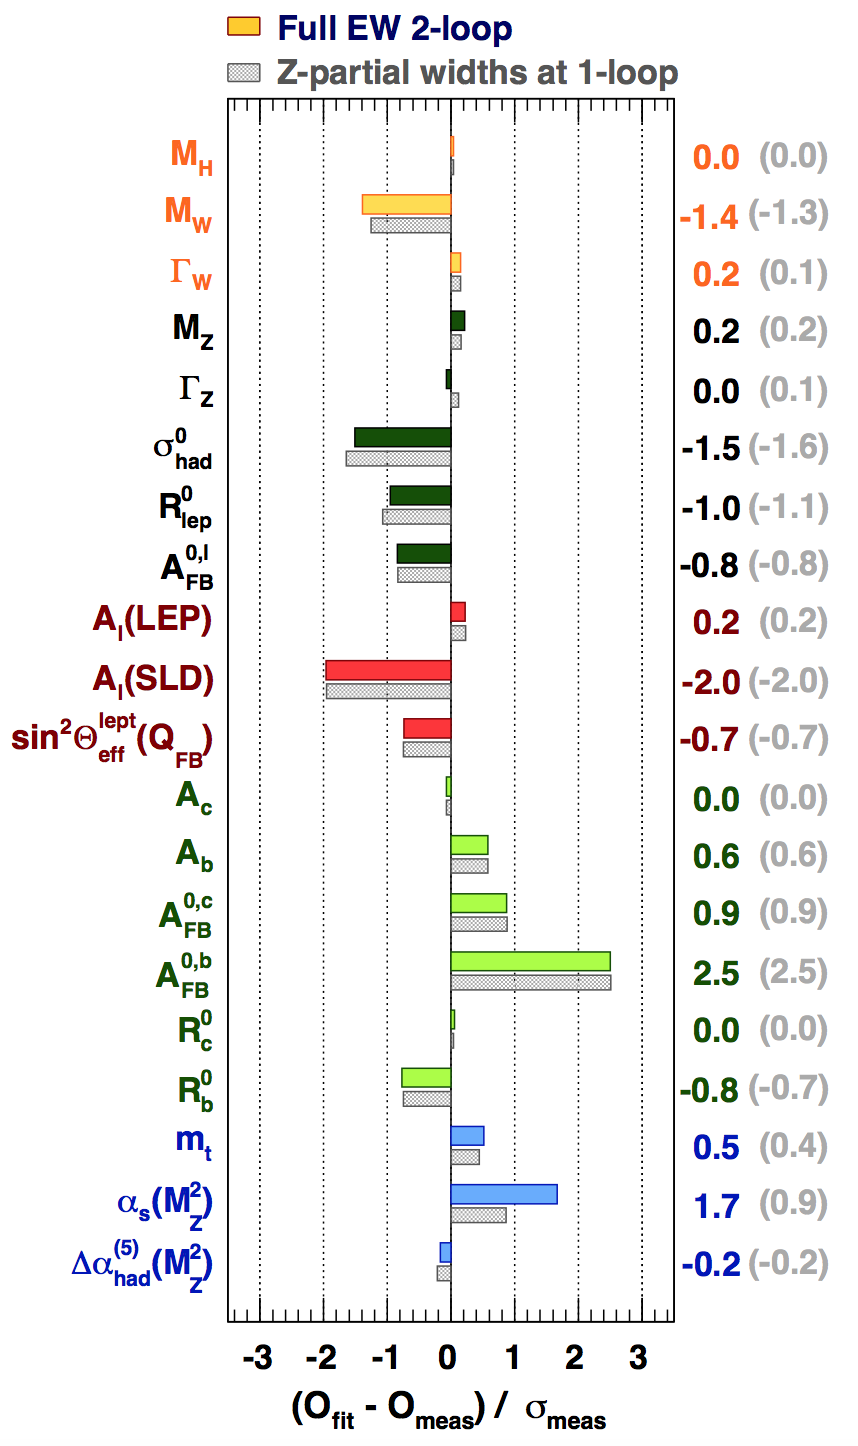
\includegraphics[width=0.75\textwidth]{\figpath/Appendix1/GFitterSMComparison.png}
    \caption{Comparison of the GFitter fit results with the direct measurements in units of the experimental uncertainty~\cite{Baak:2014ora}.}
    \label{fig:SMConsistency}
\end{figure}

\begin{figure}[!hbt]
    \centering
    \begin{subfigure}[t]{0.85\textwidth}
        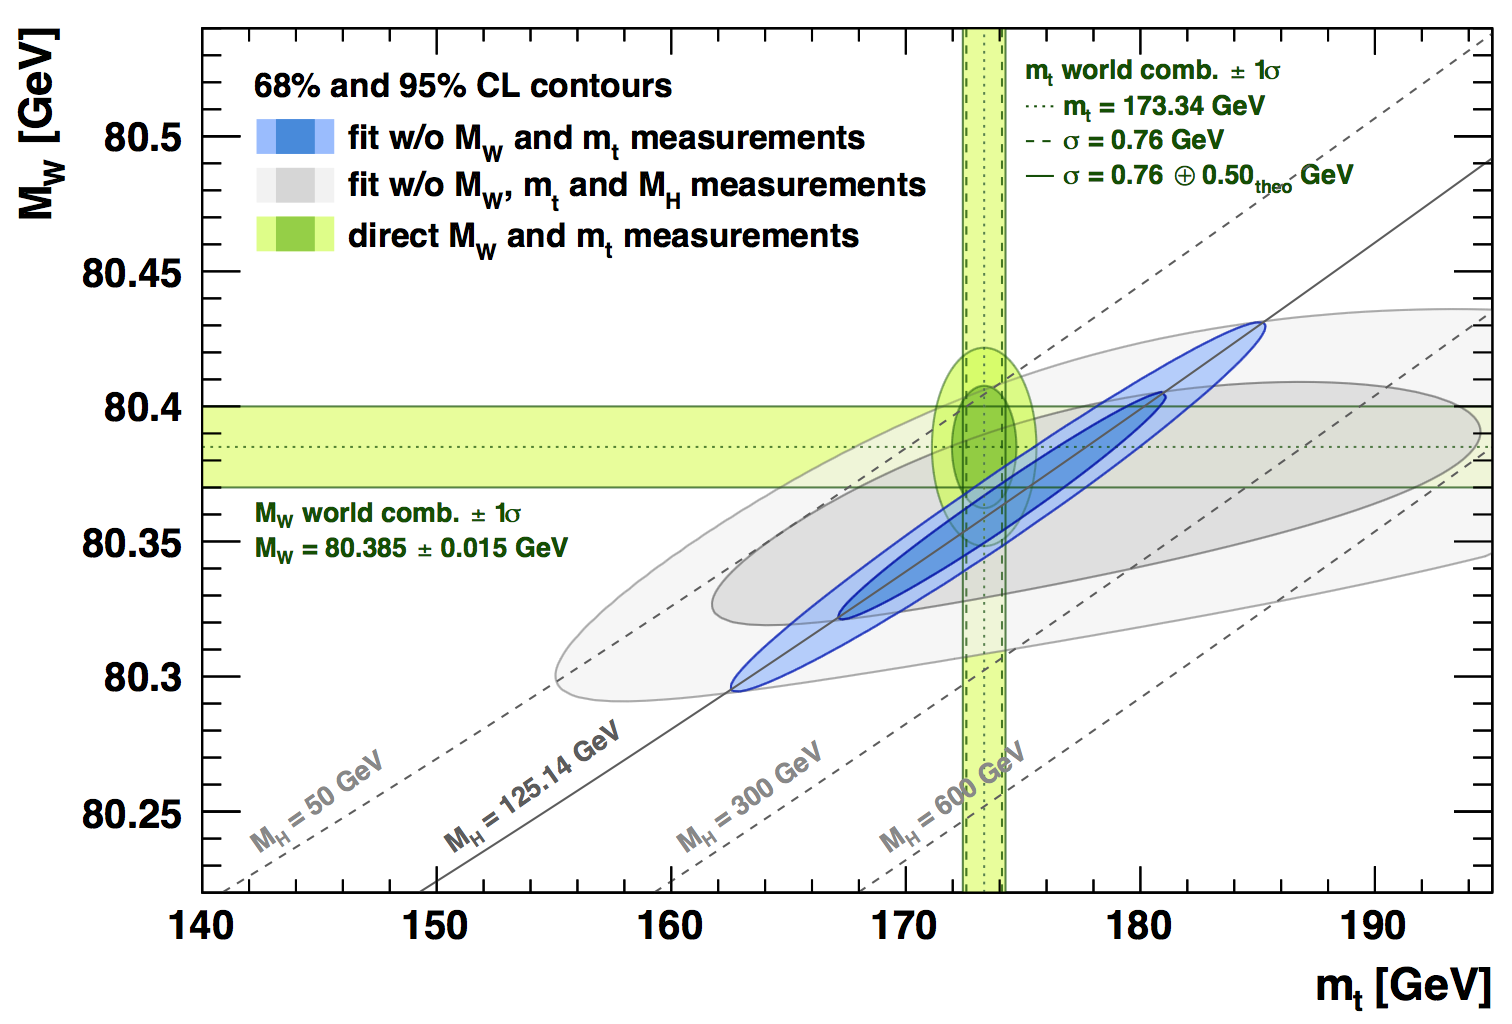
\includegraphics[width=\textwidth]{\figpath/Appendix1/GFittermWmt.png}
        \caption{}
        \label{fig:mWmtGFitter}
    \end{subfigure}

    \begin{subfigure}[t]{0.85\textwidth}
        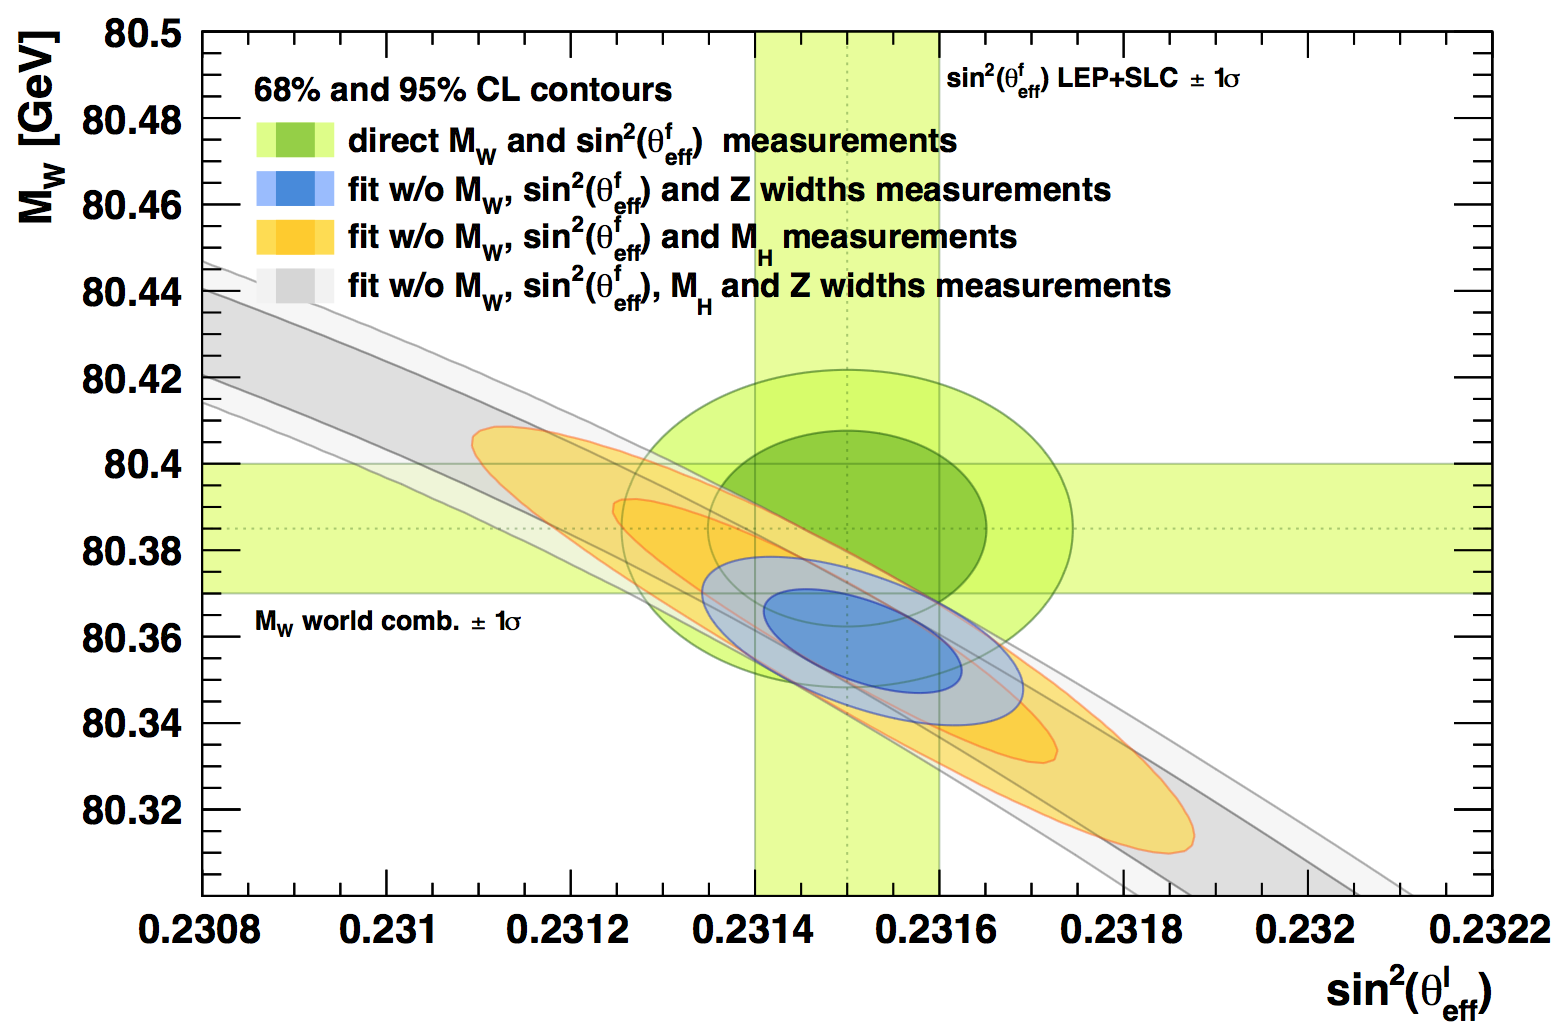
\includegraphics[width=\textwidth]{\figpath/Appendix1/GFittermWthetaEff.png}
        \caption{}
        \label{fig:mWthetaEffGFitter}
    \end{subfigure}
    \caption{Contours at 68\% and 95\% confidence level obtained from scans of \MW versus \Mt (top) and \MW versus $\sin^{2}\left(\theta_{eff}^{l}\right)$ (bottom), for a fit including \MH (blue) and excluding \MH (grey), as compared to the direct measurements (vertical and horizontal green bands and ellipses). In both figures, the corresponding direct measurements are excluded from the fit. Figure and caption from~\cite{Baak:2014ora}.}
    \label{fig:GFitterResults}
\end{figure}

